%!TeX root=../tese.tex
%("dica" para o editor de texto: este arquivo é parte de um documento maior)

% Conteúdo da subseção sobre Coortes
% Este arquivo é importado em 02-implementacao.tex

O piloto BikeSP foi estruturado como experimento controlado randomizado (RCT --- \textit{Randomized Controlled Trial}) visando responder questão de implementação fundamental (IQ1): ``Como o número de viagens de bicicleta varia com diferentes valores de remuneração?'' Esta metodologia permite isolar efeito de incentivos financeiros de fatores confundidores, fornecendo evidências causais robustas para regulamentação da Lei Municipal 16.547/2016. Participantes foram alocados a três coortes (grupos experimentais) com diferentes níveis de remuneração por quilômetro pedalado: Coorte 0 (controle, sem remuneração), Coorte 1 (incentivo baixo, R\$~0,30/km, equivalente a 1/16 da tarifa de transporte público), e Coorte 2 (incentivo alto, R\$~0,60/km, equivalente a 1/8 da tarifa). A escolha destes valores baseou-se em estudo do Banco Mundial sobre elasticidade-preço de demanda por ciclismo em São Paulo \citep{worldbank2022}, onde remunerações nesta faixa mostraram impacto significativo sem comprometer viabilidade orçamentária.

Característica distintiva do desenho foi rotação semanal de coortes: cada participante alternava entre as três condições a cada semana, experimentando todas coortes ao longo do piloto. Esta estratégia reduz viés de seleção (todos expostos a todas condições) e aumenta poder estatístico para detectar diferenças intra-indivíduos (cada participante serve como próprio controle). Adicionalmente, remuneração foi desativada em finais de semana para todas coortes, permitindo observar retenção de comportamento na ausência de incentivo financeiro --- descoberta notável foi que 9 das 10 viagens mais longas ocorreram justamente nestes períodos sem remuneração, evidência de internalização do hábito de pedalar.

A interface de coortes oferece funcionalidades para criação, listagem, e atribuição de participantes a grupos. Criação/atualização requer ID numérico único (1, 2, 3) e valor de remuneração por quilômetro; sistema automaticamente cria nova coorte se ID inexistente, ou atualiza valor se ID já cadastrado (útil para ajustes durante piloto sem recriar grupo). Listagem exibe ID, remuneração formatada como moeda (R\$~0,30), e quantidade de membros associados, com busca por ID específico e paginação (5 itens/página). Durante piloto com 1.217 participantes, distribuição manteve-se aproximadamente balanceada: ~400 participantes por coorte em qualquer semana dada, essencial para comparabilidade estatística. A Figura~\ref{fig:coortes_listagem} mostra esta interface (dados fictícios para fins ilustrativos).


 \begin{figure}[htb]
   \centering
   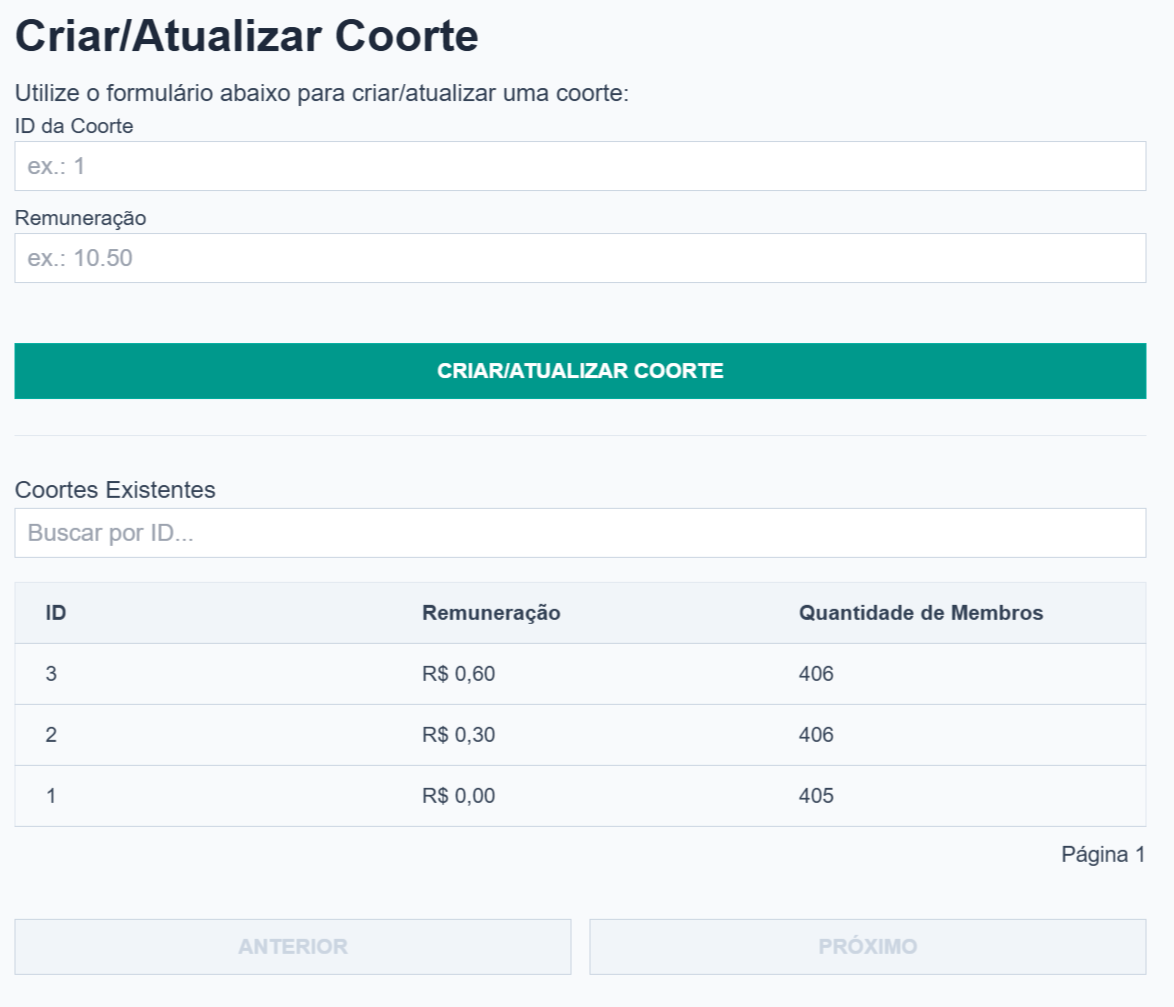
\includegraphics[width=0.95\textwidth]{figuras/coortes.PNG}
   \caption{Interface de gerenciamento de coortes e visualização de quantidade de participantes por grupo (dados fictícios).}
   \label{fig:coortes_listagem}
 \end{figure}

 A tela também contém uma tabela que lista todos usuários com respectivas coortes, exibindo ID, nome, email, total de viagens realizadas, e ID da coorte atual. Sistema de filtros combinados permite: busca por ID de pessoa, nome parcial (\textit{case-insensitive}), email, ID de coorte específica, e intervalo de viagens (mínimo/máximo). Filtros aplicam-se simultaneamente via lógica AND e persistem durante paginação. Esta funcionalidade atendeu múltiplos casos de uso: (i) verificar balanceamento de grupos (filtrar por ID de coorte, observar contagem); (ii) identificar participantes inativos (por exemplo, buscando com o filtro de usuários com no máximo 2 viagens); (iii) selecionar participantes altamente engajados para entrevistas qualitativas (por exemplo, buscando com o filtro de usuários com no mínimo 30 viagens); (iv) auditar atribuições após rotação semanal (exportar CSV, comparar com planilha esperada). A Figura~\ref{fig:coortes_listagem_usuarios} ilustra esta funcionalidade (dados fictícios para fins ilustrativos).

 \begin{figure}[htb]
    \centering
    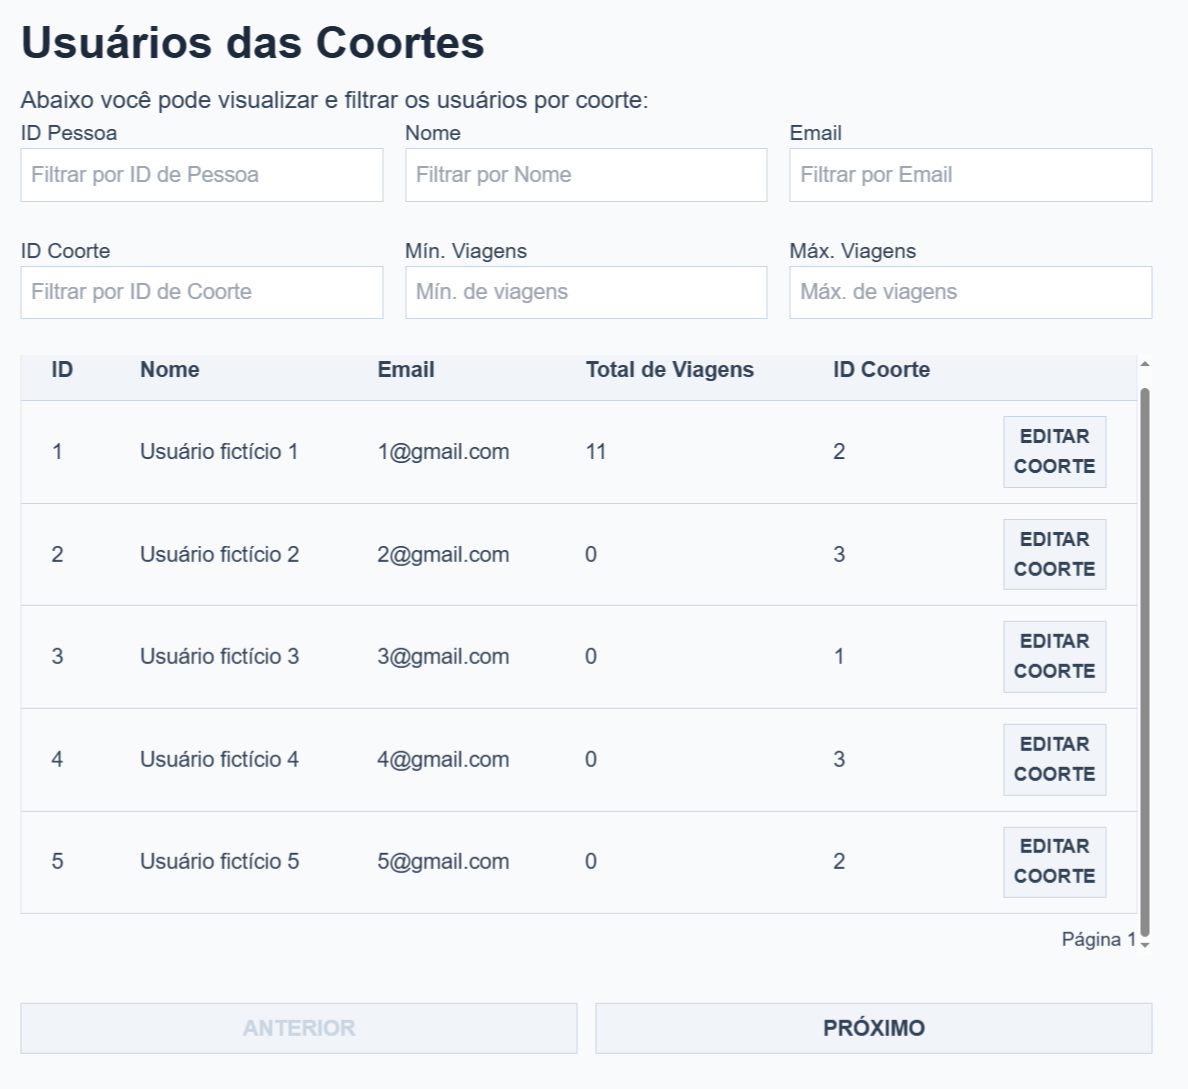
\includegraphics[width=0.95\textwidth]{figuras/usuario_coortes_zoom.PNG}
    \caption{Interface de listagem de participantes por coorte (dados fictícios).}
    \label{fig:coortes_listagem_usuarios}
  \end{figure}

Para correções pontuais, administrador pode editar coorte de usuário específico clicando ``Editar Coorte'' na linha da tabela, alterando ID para nova coorte ou deixando vazio para remover atribuição. Para operações em massa (rotação semanal), funcionalidade de upload via CSV permite atribuições em lote: arquivo com duas colunas (CPF;ID\_Coorte) separadas por ponto-e-vírgula, sem cabeçalho, codificação UTF-8. Sistema valida linha por linha antes de processar: CPF deve existir, coorte destino deve estar cadastrada, CPFs não podem duplicar. Erros específicos (``CPF 12345678901 não encontrado'', ``Coorte 99 não existe'') facilitam correção e reupload. Processamento atômico garante que ou todas atribuições são aplicadas ou nenhuma, prevenindo estados parciais que comprometeriam integridade experimental.

Durante piloto, rotação semanal típica seguia workflow: economistas geravam CSV com nova atribuição usando script (randomização estratificada por perfil socioeconômico e localização geográfica); administrador fazia upload via painel (Figura~\ref{fig:coortes_listagem_upload}); sistema atualizava os registros; notificações push/email informavam participantes sobre nova remuneração vigente; exportação CSV pós-upload confirmava aplicação correta. Este processo de rotação semanal ao longo do projeto piloto evidenciou robustez e eficiência da funcionalidade.

\begin{figure}[htb]
    \centering
    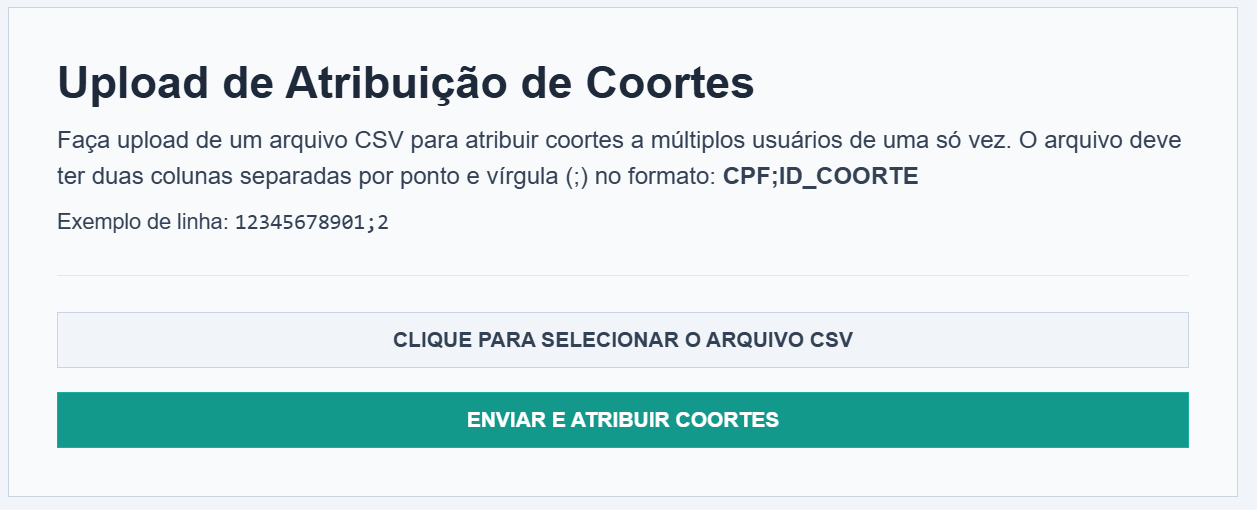
\includegraphics[width=0.95\textwidth]{figuras/upload_coortes.PNG}
    \caption{Interface de upload de atribuição de coortes em lote.}
    \label{fig:coortes_listagem_upload}
  \end{figure}

O botão de exportação gera CSV completo com ID, nome, CPF, email, ID da coorte, e valor de remuneração atual. O formato compatível com ferramentas estatísticas e facilita análises, o nome do arquivo gerado inclui a data da exportação, importante para criar um histórico versionado. A Figura~\ref{fig:coortes_listagem_exportar} mostra esta funcionalidade.

\begin{figure}[htb]
    \centering
    
\includegraphics[width=0.95\textwidth]{figuras/exportar_coortes.PNG}
    \caption{Interface de exportação de coortes.}
    \label{fig:coortes_listagem_exportar}
  \end{figure}

O sistema implementa múltiplas salvaguardas: coortes não podem ser deletadas se possuem membros (previne perda acidental de atribuições); mudanças de remuneração em coorte ativa geram log detalhado (rastreabilidade de alterações durante experimento); tentativas de atribuir participante a coorte inexistente são rejeitadas (impossibilita referências órfãs); exportações registram data, horário e usuário que solicitou (auditoria de acesso a dados sensíveis).

A infraestrutura de gerenciamento de coortes no painel viabilizou análises sobre o impacto diferencial das remunerações. Os dados coletados durante o piloto permitirão investigar relações dose-resposta (comparando número de viagens entre diferentes valores de remuneração), validar a estratégia de rotação semanal, examinar retenção de participantes em cada coorte, e explorar heterogeneidade de efeitos por perfis socioeconômicos. Estas descobertas fundamentarão documento de recomendações para regulamentação da Lei Municipal 16.547/2016.


